%!TEX root = index.tex
\section{Cycle de développement logiciel}

Les cycles de développement des systèmes dans l'ingénierie des systèmes sont les processus de création ou de modification de systèmes d'information et les modèles et méthodes utilisés pour développer ces systèmes. En génie logiciel, ce concept sous-tend de nombreux types de méthodologies, et ces méthodes constituent le cadre pour la planification et le contrôle de la création d'un système d'information \cite{cycle}.

\begin{figure}[h]
\begin{center}
    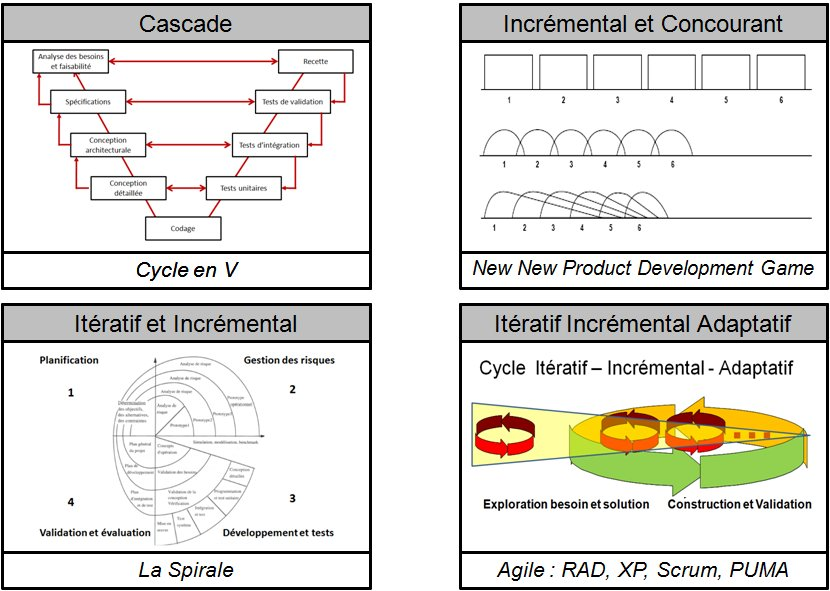
\includegraphics[scale=0.4]{img/cycles-basiques}
    \caption{Les principales cycles de développement logiciel}
	\label{cycles-basiques}
\end{center}
\end{figure}

..Du point de vue d'un projet nouveau et de la gestion de projets, normalement les étapes exécutées par l'équipe étaient la . Toutefois, comme j'ai rejoint le projet dans son milieu, je n'ai pas pu assister à toutes les étapes de conception  
